\chapter{State of the Field}
Unfortunately, there is not a great deal of scientific research into communication products for nonverbal autistic children. Luckily, however, this field is closely connected to other fields that have a great deal of research, such as human-computer interaction, effective learning techniques of children with nonverbal autism and the effects of the disorder, and nonverbal communication.  By combining these areas of related research with the current solutions in the field, an accurate depiction of the current state of the field can be built and used to further research in this area.
\subsection{Related Research}
\subsubsection{Nonverbal Human Communication Research}
While this research is not directed at those with autism, nonverbal human communication has been heavily researched and can provide key insights that may help influence the development of our application. Humans rely heavily on nonverbal communication in the forms of body language, tone, and gestures. It has been proven that there are patterns to nonverbal communication that can give incredible insights into the conversation. One study was able to take a small window of a group interaction and determine the social dynamic and map emotions to individuals by analyzing only nonverbal interactions~\cite{jayagopi}. By studying human-to-human nonverbal interactions, frameworks have been built that allow computers to read emotions and intentions based on only nonverbal input~\cite{sumi}. Since eye contact and facial expressions are difficult for nonverbal autistic children to both decipher and communicate, this research could be applied to our application in order to facilitate a more natural feeling conversation for the teacher or peer communicating with the autistic child or to help give the child context relating to the conversation that they otherwise may not realize.

\subsubsection{Human-Computer Interaction Research}
Human-Computer Interaction has also been heavily researched. Based on the large data set of human interactions, human-computer interactions have been developed that feel natural~\cite{rich} and conversational models can be built from this data that assist in making computers seem more human-like. These frameworks can be applied to assist in human-to-human interactions as well~\cite{sumi}.
\subsubsection{Autistic Children Education Research}
While research on the effects of specific products or applications on the education of children with autism is lacking, there is plenty of research on education techniques in general. Specifically relevant to our idea are claims that technology improves education for children with autism and that graphics are more easily understood than text.
\begin{enumerate}\bfseries
\item Autistic children learn more effectively through the use of technology.
\begin{itemize}
\item  \textnormal{Moore and Calvert proved that using technology with children with autism is more effective than single teacher instruction with no technology~\cite{moore}.}
\item  \textnormal{Goldsmith and LeBlanc proved that technology is effective in treating the symptoms and social effects of autism~\cite{goldsmith}.}
\item  \textnormal{Some teachers believe that technology levels the playing field between nonverbal and verbal students by making nonverbal methods of communication using technology more ?normal? or even more ?cutting edge,? changing the classroom dynamic and stigma around students with disabilities~\cite{riechmann}.}
\end{itemize}
\item Autistic children  understand visual and auditory aids much more easily than text.
\begin{itemize}
\item  \textnormal{Pictures improve reading and comprehension skills and increases engagement in students with disabilities~\cite{slater}.}
\item  \textnormal{Sound and visual effects engage autistic children more effectively in the classroom~\cite{moore}.}
\item  \textnormal{Some believe that the reason technology is so effective in educating and engaging children with autism is due to auditory and visual prompts, especially video~\cite{goldsmith}.}
\item  \textnormal{The fading technique, which entails slowly removing contextual graphic cues until only a word is left behind, and found that children with autism who could initially use the logos eventually were able to use the orthographic symbols, or letters, proving that the visuals are effective in transitioning towards text~\cite{hetzroni}.}
\end{itemize}
\end{enumerate}

\subsection{Related Patents}
Several related technologies and techniques have been patented in the United States. Below, we highlight two of the most relevant patents to our research and development of the application. We also discuss why we believe neither of these patents will conflict with our application.

\subsubsection{Interactive systems employing robotic companions (Granted)}
This patent covers an interactive robotic companion that could be used in any activity involving the user. While this is a fairly general explanation, the patent goes on to give examples of applications for this technology, one of which includes "a system for communicating with patients that have difficulties communicating verbally" \cite{stiehl}. While this is very similar to what we will try to accomplish in our application, our application will be created for a tablet or phone, while this patent suggests that the program would be run on a robot capable of touch and sensing its environment.

\subsubsection{Method and system for communication using a portable device (Pending)}
This patent covers a system of communication in which the first user is given a choice of options to select to communicate, and, upon the first user selecting one of the given options, the system communicates the message to a second user in another format~\cite{rashdan}. This idea, which is still pending patent approval, would conflict with our product, but it is such a general patent that it would also conflict with almost every communication app on the market today. In addition to conflicting with other Augmented-Alternative Communication apps (AAC), even something as simple as the the word suggestions in Apple's iMessage application, or the stickers in Facebook's Messenger could be seen as conflicting with this patent. Because of its generality and pending status, we will ignore this patent for now and revisit it when we are closer to the release date in May.

\subsection{Existing Applications}

\subsubsection{Look in My Eyes: Steam Train}
The Look in My Eyes: Steam Train application is a fun game-based app that is supposed to help the user practice eye contact. It is designed as a non-competitive game and consists of multiple levels and mini-games that all focus on the same objective. The user interface, shown in Fig.~{fig:lookInMyEyes}, is bright and graphical, making it easy to use for many age groups and cognition levels. The app is available on the Apple App Store for \$2.99~\cite{lookInMyEyes}.

\begin{figure}[!htb]
\centering
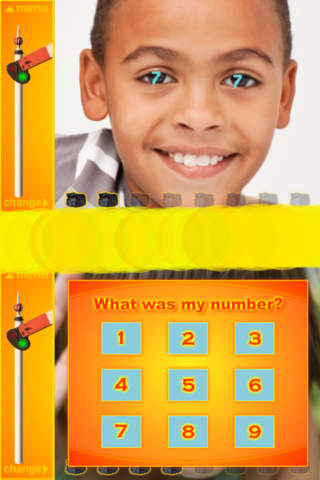
\includegraphics[width=.6\textwidth]{lookInMyEyes.png}
\caption{\label{fig:lookInMyEyes}Screenshot of the Look In My Eyes: Steam Train application user interface}
\end{figure}

\subsubsection{Communicate Easy}
This application aims to help users formulate sentences via a picture-based user interface (Fig.~\ref{fig:communicateEasy}). It is successful in providing an easy learning curve for new users because of the simple user interface design. It includes the ability for a user to develop their own icons for the buttons that trigger the audio playback. This application is listed for \$2.99 and is only available on iOS devices~\cite{communicateEasy}.


\begin{figure}[!htb]
\centering
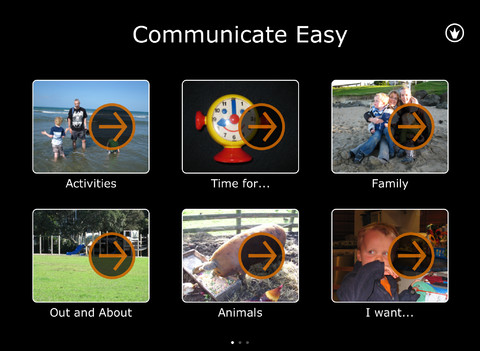
\includegraphics[width=.7\textwidth]{communicateEasy.jpg}
\caption{\label{fig:communicateEasy}Screenshot of the Communicate Easy application user interface}
\end{figure}

\subsubsection{Keeble}
Keeble is an iOS accessible keyboard for the iPad, iPhone, and iPod touch. The keyboard can be used within any app on an iOS device and is designed to enable people with physical or visual impairments to type more easily. It can be customized to the individual's preferences, as shown in Fig.~\ref{fig:keeble}, and offers word prediction, timing options, Select on Release, Select on Dwell, auditory feedback and other accessibility features. The keyboard add-on is  offered for \$24.99 on Apple's App Store~\cite{keeble}.

This application was featured in an Apple television advertisement of a young man who is both autistic and non-verbal, who was able to begin expressively communicating via apps on his iPad.

\begin{figure}[!htb]
\centering
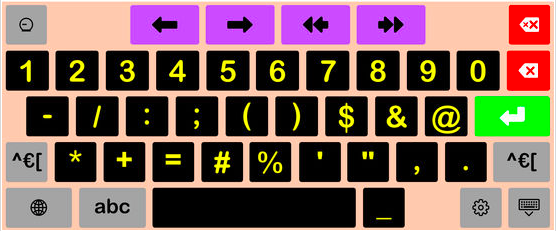
\includegraphics[width=1\textwidth]{keeble.png}
\caption{\label{fig:keeble}Screenshot of one of the Keeble keyboard configuration options}
\end{figure}

\subsubsection{SPEAKall!}
The SPEAKall! application, which is shown in Fig.~\ref{fig:speakAll}, is a popular application for people of all ages living with autism. The application teaches vocabulary and sentence construction, while maintaining a fun and engaging user experience. It won the 2015 Outstanding Research of the Year Award from the Autism Society.

The application is only available on iOS devices and is listed at \$39.99 on the App Store~\cite{speakAll}. 

\begin{figure}[!htb]
\centering
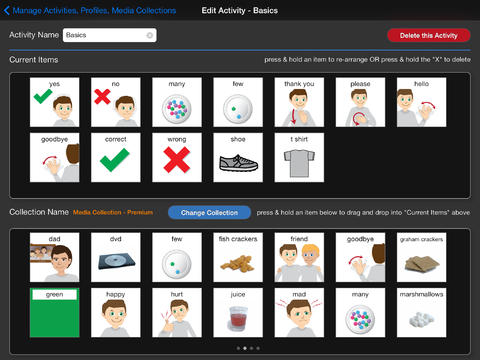
\includegraphics[width=.7\textwidth]{speakAll.png}
\caption{\label{fig:speakAll}Screenshot of the SPEAKall! application user interface}
\end{figure}

\subsubsection{Proloquo2Go}
Proloquo2Go, shown on the Apple iPad in Fig.~\ref{fig:proloquo2go}, is an award-winning symbol-supported communication app. The app is designed to promote language development in users at any level and grow communication skills through use. It allows users to quickly personalize the vocabulary and settings of the application, and it is listed for \$249.99 on the App Store~\cite{proloquo}. 

\begin{figure}[!htb]
\centering
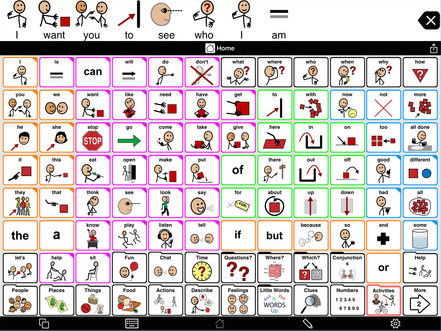
\includegraphics[width=.6\textwidth]{proloquo2go.png}
\caption{\label{fig:proloquo2go}Screenshot of the Proloquo2Go application user interface}
\end{figure}